% ============================================================================
% 中文注释：第 4 节 失败模式（2026-11-03 重写为四小节 + 区域项）
% ----------------------------------------------------------------------------
% 4.1 Ω 内所有方法劣于不作处理（表 1 + 图 2）
% 4.2 损伤是"结构"不是"光度"；而且没有任何方法打赢"无内容先验的平滑上限"
% 4.3 反射与场景同频段 ⇒ 搬高频反而掉分（解释为什么滤波/感知都无效）
% 4.4 残余光度误差是逐图的、不可跨场景迁移（P4 的量化）
% 4.5 起决定作用的损失项不是"区域"，而是"相对归一"（随机盘对照）
% 关键数字：
%   identity 24.52；公开 20.9–23.6；我们 22.30/22.39
%   结构保有率 identity 1.14 / quiet 0.65 / 50:50 0.48
%   MAE_aff identity 10.51 / quiet 11.70 / 50:50 10.71
%   平滑上限：弱区 29.50（identity 31.45，quiet 27.18）；强区 15.24（identity 14.46，quiet 13.48）
%   高频拼接：quiet 22.26→22.04(σ=2)→21.66(σ=4)；50:50 23.73→23.39
%   Δaff：identity 1.94 / RDNet 1.00 / 我们 0.15–0.26；共享 0.50 / 0.59 / 0.07
%   λ_om=0 → 18.33；随机盘 19.90 > 真掩码 19.41 > 无区域项 17.76
% ============================================================================
\section{Where SIRR Fails on Tinted Glass}
\label{sec:diagnosis}

% ============================================================================
% 中文注释：表 1 主结果（跨双栏 table*）
% ----------------------------------------------------------------------------
% 口径：15 场景、**手标 Ω** 掩码、存盘 uint8 PNG、同一冻结评测脚本。
% 行：
%   identity            —— 什么都不做（分数地板）；Ω 内 24.52 是全场最高，这是本文的核心事实
%   IBLCN / ERRNet / LightRR / RDNet(0-shot) / DSRNet / Zhu24 —— 六个公开方法，全部零样本
%   Ours (baseline)     —— 我们的 9 项损失基线，三种子 22.49±0.44
%   Ours + L_quiet      —— 本文的方法，三种子 22.99±0.34
% 列说明：
%   ΔΩ = PSNR_Ω(方法) − PSNR_Ω(identity)，**全是负的**（=所有方法都在 Ω 内比不动更差）
%   β  = 残留反射系数（−1 没去、0 完美）；公开方法的预测我们没有 R 分支，故留 "—"
%   α  = 逐图增益中位数（1 = 亮度对；偏离说明模型只是在整体提亮/压暗）
% 注意：
%   1) Ω 内/外的绝对值不可直接比（Ω 更暗、PSNR 偏爱暗区），必须看 ΔΩ；
%   2) 最佳值加粗：PSNR_Ω 与 ΔΩ 用 identity，PSNR 用我们的 L_quiet；
%   3) 细节指标（HF-PSNR、梯度余弦、LapVar）用来防"糊出来的 PSNR"——我们的 LapVar 只有 GT 的 0.6。
% ============================================================================
\begin{table*}[t]
\centering
\caption{Main results on the $15$-scene tinted-glass panel. $^\dagger$: three seeds,
mean$\pm$sd over scenes. $\Delta_\Om$ is measured \emph{against identity inside $\Om$}
(Eq.~1); it is negative for every method. $\beta$: residual-reflection coefficient
($-1$: nothing removed, $0$: perfect). $\alpha$: median per-image gain. The best value in each
column is in bold.}
\label{tab:main}
\setlength{\tabcolsep}{4pt}
\small
\begin{tabular}{lcccccccc}
\toprule
Method & PSNR$\uparrow$ & SSIM$\uparrow$ & HF-PSNR$\uparrow$ & grad-cos$\uparrow$ & LapVar & PSNR$_\Om\uparrow$ & $\Delta_\Om$ & $\beta$$\downarrow$ \\
\midrule
Identity (no removal)      & 18.44 & 0.693 & 32.96 & 0.599 & 52.5 & \textbf{24.52} & $0.00$ & $-1.00$ \\
IBLCN~\cite{li20}          & 18.12 & 0.683 & 32.68 & 0.582 & 61.0 & 23.55 & $-0.97$ & --- \\
ERRNet~\cite{wei19}        & 18.90 & 0.710 & 33.64 & 0.614 & 25.8 & 22.97 & $-1.55$ & --- \\
LightRR~\cite{lightrr26}   & 19.18 & 0.680 & 32.34 & 0.594 & 68.8 & 20.89 & $-3.63$ & --- \\
RDNet~\cite{rdnet25} (0-shot) & 20.05 & 0.728 & 33.87 & 0.611 & 30.8 & 21.32 & $-3.20$ & $-0.59$ \\
DSRNet~\cite{dsrnet24}     & 20.25 & 0.732 & 33.93 & 0.622 & 21.6 & 21.95 & $-2.57$ & --- \\
Zhu~\cite{zhu24}           & 20.50 & 0.735 & 33.83 & 0.605 & 31.5 & 21.37 & $-3.15$ & --- \\
\midrule
Ours (baseline)$^\dagger$  & 22.49$\pm$0.44 & 0.773 & 34.33 & 0.604 & 23.8 & 22.30 & $-2.22$ & $-0.29$ \\
\textbf{Ours + $\quiet$}$^\dagger$ & \textbf{22.99}$\pm$0.34 & \textbf{0.778} & \textbf{34.42} & \textbf{0.610} & 23.4 & 22.39 & $-2.13$ & $-0.34$ \\
\bottomrule
\end{tabular}
\end{table*}


% 中文：定性图——两场景 × [I, GT, 预测, |误差|]，Ω 用红/绿轮廓标出。
\begin{figure}[t]
\centering
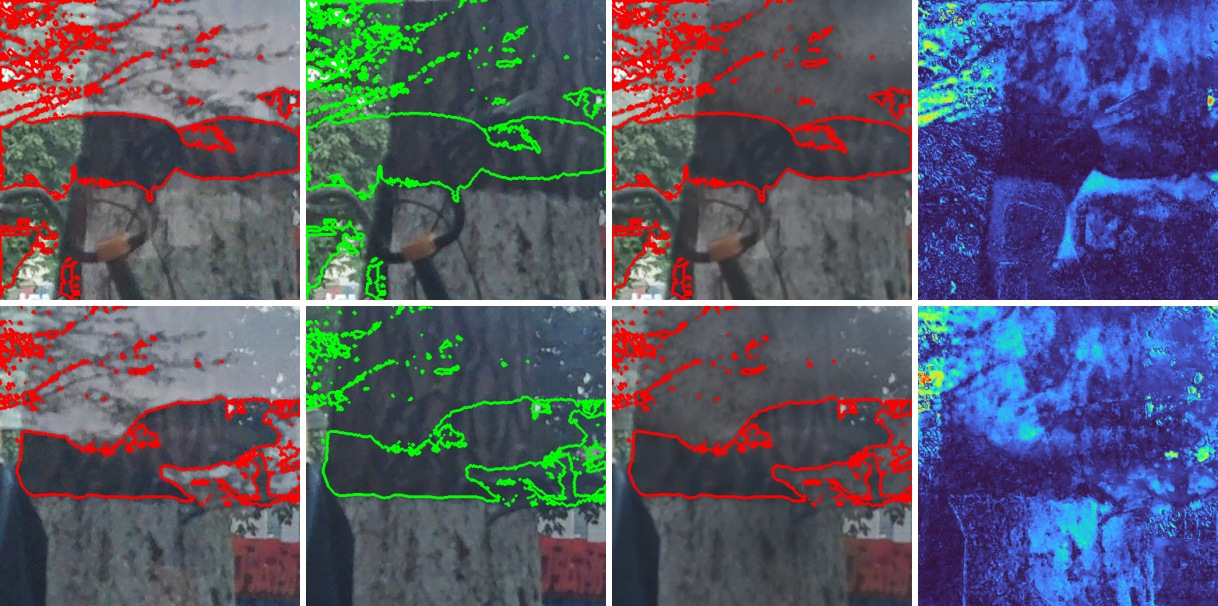
\includegraphics[width=\linewidth]{fig/qual_omega.jpg}
\caption{\textbf{Where the damage happens.} Two scenes (rows). Columns: input $I$; ground
truth $T$; our prediction; absolute error $|\That-T|$ (turbo, per-image normalised).
Red/green contours: the hand-annotated occluder region $\Om$. The error map lights up
\emph{along the occluder} rather than in the reflected content---the signature of a
``remove reflection'' prior applied where there is little reflection to remove.}
\label{fig:qual}
\end{figure}

\subsection{$\Om$ needs almost no change; its \emph{neighbourhood} does}
\label{sec:axis1}

The occluder region $\Om$ is not where the reflection is strongest---it is where it is weakest.
Partitioning each frame into $\Om$, a $15$\,px annulus around it, and the remaining far field gives
three bands that behave completely differently:

\begin{center}
\small
\setlength{\tabcolsep}{3pt}
\begin{tabular}{@{}lccccc@{}}
\toprule
band & area & $\mathbb{E}|I-T|$ & refl./trans. & identity & $+\quiet$ \\
\midrule
$\Om$ itself        & ---    & $\mathbf{10.3}$ & $0.112$ & $24.49$ & $22.26$ ($-2.23$) \\
\textbf{annulus ($15$\,px)} & $44.4\%$ & $\mathbf{44.4}$ & $\mathbf{0.516}$ & $13.76$ & $19.44$ ($\mathbf{+5.68}$) \\
far field           & ---    & $16.8$ & $0.164$ & $19.52$ & $23.53$ ($+4.02$) \\
\bottomrule
\end{tabular}
\end{center}

(PSNR is computed within each band, so bands are not comparable to one another; the informative
quantity is each model against identity \emph{within} a band.)

Three readings. \emph{(a)} The reflection in the annulus is $4.3\times$ stronger than inside $\Om$
and $2.6\times$ stronger than in the far field: the strong reflection does not sit \emph{in} the
occluder region, it sits \emph{next to} it. \emph{(b)} The annulus is not a fringe---it covers
$44\%$ of the frame---and it is where the models' absolute quality is worst ($19.4$--$19.8\dBA$
versus $23.5$ far away). \emph{(c)} Inside $\Om$ every method is worse than doing nothing
($-2.2\dBA$), because almost nothing needs to change there ($10.3$ gray levels) and the model
changes it anyway.

% 中文：这条把"边界为什么显眼"讲清楚——不是 Ω 内坏了，是紧邻的强反射带质量最差，
% 而它贴着 Ω，人眼一对比就看出来了。要修它必须靠长程语义连续（例如左下角的树干下半段）。
The consequence is perceptual rather than numerical: the annulus abuts a region that is already
almost correct, so its residual error is read by the eye as a \emph{boundary}. Fixing it is not a
matter of removing more reflection---the transmitted structure there is buried, and recovering it
requires extrapolating from content elsewhere in the frame along semantic continuations (a tree
trunk continued from its lower part, a railing continued from the left). This is the cloze-like
regime of Sec.~\ref{sec:band}, and it is the one failure mode no method we tested addresses.

\subsection{The damage is structural, and no model beats a blur}
\label{sec:structural}
\label{sec:ceiling}

A photometric explanation would predict that the models merely mis-scale $\Om$. They do
not. Restricting to $\Om$ and allowing a \emph{per-image affine correction} before
scoring, models keep only a fraction of the ground-truth structure:

\begin{center}
\small
\setlength{\tabcolsep}{4pt}
\begin{tabular}{@{}lcccc@{}}
\toprule
 & identity & base & $+\quiet$ & 50:50 \\
\midrule
structure retained (LapVar ratio) & $1.14$ & $0.50$ & $\mathbf{0.65}$ & $0.48$ \\
MAE, per-image affine-corrected & $10.51$ & $12.82$ & $11.70$ & $\mathbf{10.71}$ \\
\bottomrule
\end{tabular}
\end{center}

Two readings. First, the mixed model's affinity-corrected error ($10.71$) is essentially
identity's ($10.51$) while its structure is halved---it ``wins'' the error metric by
flattening $\Om$. Second, we can bound what any content-agnostic method can do: smoothing
the input with a Gaussian is the best a model can achieve if it knows nothing about the
content. On the weakly-reflected $59\%$ of $\Om$ that ceiling is $29.50\dBA$, against
identity's $31.45$ and $\quiet$'s $27.18$; on the strongly-reflected $7\%$ it is
$15.24\dBA$, against $14.46$ (identity) and $13.48$ ($\quiet$). \textbf{No model we
trained beats a plain blur, in either regime.}

\subsection{Reflection and scene share the frequency band}
\label{sec:band}

$34.5\%$ of the reflection's energy lies above a $\sigma{=}8$ low-pass, so it is not a veil
that can be filtered away. We verified the consequence directly: replacing the low
frequencies of a model output with those of the model and the high frequencies with those
of the \emph{input},
$\That' = \mathrm{LP}_\sigma(\That) + \big(I-\mathrm{LP}_\sigma(I)\big)$, inside $\Om$
restores structure fidelity ($1.31\times$ at $\sigma{=}2$) but \emph{lowers} PSNR:

\begin{center}
\small
\setlength{\tabcolsep}{4pt}
\begin{tabular}{@{}lccc@{}}
\toprule
PSNR in $\Om$ & plain & $+\,\sigma{=}2$ & $+\,\sigma{=}4$ \\
\midrule
$+\quiet$ & $22.26$ & $22.04$ & $21.66$ \\
50:50 & $23.73$ & $23.39$ & $22.97$ \\
\bottomrule
\end{tabular}
\end{center}

The band that carries the missing structure also carries the reflection. Separating the
two is not a filtering problem; it requires knowing which structures belong to the scene,
i.e.\ a semantic prior. This is also why a perceptual loss does not help: it is
\emph{mean-seeking}, so under the layer ambiguity of Eq.~\eqref{eq:film} it averages the
plausible completions and produces the conservative ``hedged'' output we observe.

\subsection{What survives fine-tuning is per-image}
\label{sec:photometric}

We measure two photometric oracles: a per-image affine fitted on that image's ground
truth, and a single shared affine fitted on the other $14$ scenes (leave-one-scene-out).
Their gap is the part any cross-scene rule could remove.

\begin{center}
\small
\setlength{\tabcolsep}{4pt}
\begin{tabular}{lcc}
\toprule
 & per-image oracle & shared (LOO) \\
\midrule
identity & $+1.94$ & $+0.50$ \\
RDNet (zero-shot) & $+1.00$ & $+0.59$ \\
ours (fine-tuned) & $+0.15$--$0.26$ & $+0.07$ \\
\bottomrule
\end{tabular}
\end{center}

Fine-tuning consumes the transferable part ($0.59\rightarrow0.07\dBA$) and leaves a
residual that is per-image. Any module estimating a global photometric quantity from a
single frame is therefore bounded by $0.07\dBA$---which is why the $8{\times}8$ adapter and
the input-side rescaling of Sec.~\ref{sec:negative} both failed.

\subsection{The load-bearing term is not about the region}
\label{sec:axis3}

Our loss contains a region-relative error inside $\Om$,
\begin{equation}
\reg=\lambda_{\Om}\,\mathbb{E}_{\Om}\!\left[\,
\frac{|T-\That|}{\mathbb{E}_{\Om}|T-I|}\ \right].
\label{eq:lom}
\end{equation}
Removing it is catastrophic---PSNR falls from $22.49$ to $18.33\dBA$, i.e.\ \emph{below}
identity ($18.44\dBA$)---so by any ablation it is the single most important term of a
nine-term objective. Its power, however, is not the annotation. Replacing the hand mask by
a random disk of equal area (three seeds, separate $82$-pair pool) gives

\begin{center}
\small
\setlength{\tabcolsep}{4pt}
\begin{tabular}{lcc}
\toprule
region used in Eq.~\eqref{eq:lom} & PSNR & seed sd \\
\midrule
none ($\lambda_\Om=0$) & $17.76$ & $0.16$ \\
hand-annotated $\Om$ & $19.41$ & $0.54$ \\
\textbf{random disk} & $\mathbf{19.90}$ & $\mathbf{0.16}$ \\
\bottomrule
\end{tabular}
\end{center}

% 中文：这条说明为什么"紧凑区域 + 高权重"在这里需要而在普通 SIRR 里不需要。
% 注意：这是**由覆盖率统计支撑的推断**，不是在公开数据上训出来的结论，行文里要标明。
\paragraph{Why a compact, high-weight region helps here and not in standard SIRR.}
We do not claim this as a training result on public data; we state it as an inference supported by
coverage statistics. Defining the reflection's spatial \emph{coverage} as the fraction of pixels
whose residual exceeds $15\%$ of its 90th percentile, the median coverage is $83.5\%$ on
SIR$^2$ ($499$ pairs), $70.6\%$ on Real20 ($109$ pairs) and only $52.7\%$ on our filmed panel. When
the reflection covers almost the whole frame, a global $L_1$ already carries a separation signal
everywhere and no extra term is needed. When it covers half the frame, the global loss is dominated
by pixels for which ``do nothing'' is nearly optimal (inside $\Om$, $\mathbb{E}|I-T|=10.3$ gray
levels), and a compact region with a large weight is what puts the gradient back. This is also why
region-weighted losses are routine in \emph{sparse}-degradation restoration---deraining, scratch and
shadow removal---while being essentially absent from the SIRR literature: existing SIRR data is
dense, and there is nothing for them to expose.

A random disk is not only as good, it \emph{stabilises} training. The benefit of
Eq.~\eqref{eq:lom} is the relative normalisation---being accurate in a compact region
despite little change being needed---not region recognition. Sec.~\ref{sec:method} turns
this into a mask-free regularizer.
